\documentclass[12pt,letterpaper]{article}
\usepackage{fullpage}
\usepackage[top=2cm, bottom=4.5cm, left=2.5cm, right=2.5cm]{geometry}
\usepackage{amsmath,amsthm,amsfonts,amssymb,amscd}
\usepackage{lastpage}
\usepackage{enumerate}
\usepackage{fancyhdr}
\usepackage{mathrsfs}
\usepackage{xcolor}
\usepackage{graphicx}
\usepackage{listings}
\usepackage{hyperref}
\usepackage{amsmath}
\usepackage{mathtools}
\usepackage{tikz}
\usepackage{array}
\usetikzlibrary{matrix}

\hypersetup{%
  colorlinks=true,
  linkcolor=blue,
  linkbordercolor={0 0 1}
}
 
\renewcommand\lstlistingname{Section}
\renewcommand\lstlistlistingname{Algorithms}
\def\lstlistingautorefname{Alg.}

\lstdefinestyle{Python}{
    language        = Python,
    frame           = lines, 
    basicstyle      = \footnotesize,
    keywordstyle    = \color{blue},
    stringstyle     = \color{green},
    commentstyle    = \color{red}\ttfamily
}

\setlength{\parindent}{0.0in}
\setlength{\parskip}{0.05in}

% Edit these as appropriate
\newcommand\course{CSE 3500}
\newcommand\hwnumber{1}                  % <-- homework number
\newcommand\NetIDa{rjf23002}           % <-- NetID of person #1
\newcommand\NetIDb{}           % <-- NetID of person #2 (Comment this line out for problem sets)

\pagestyle{fancyplain}
\headheight 35pt
\lhead{\NetIDa}
\lhead{\NetIDa\\\NetIDb}                 % <-- Comment this line out for problem sets (make sure you are person #1)
\chead{\textbf{\Large Homework \hwnumber}}
\rhead{\course \\ \today}
\lfoot{}
\cfoot{}
\rfoot{\small\thepage}
\headsep 1.5em

\begin{document}

\section*{Benchmarking}

\begin{figure}[!h]
  \centering
  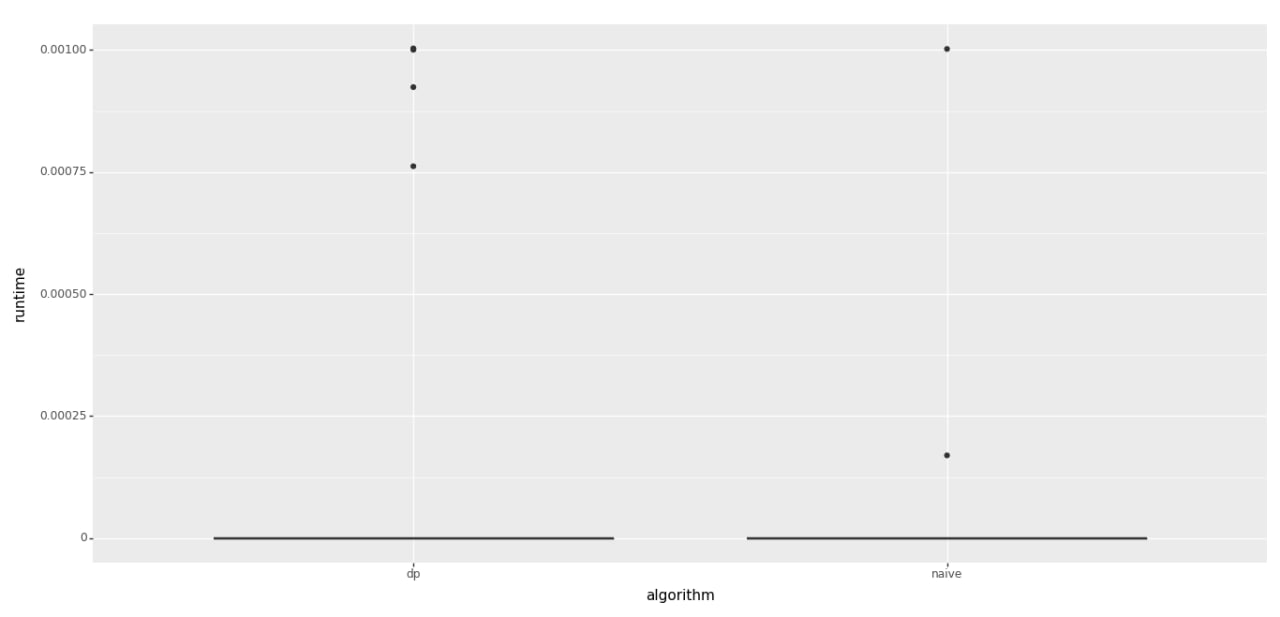
\includegraphics[width=1.0\linewidth]{benchmark_3x3.jpg}
  \caption{Benchmark on a 3x3 image.}
  \end{figure}

\begin{figure}[!h]
  \centering
  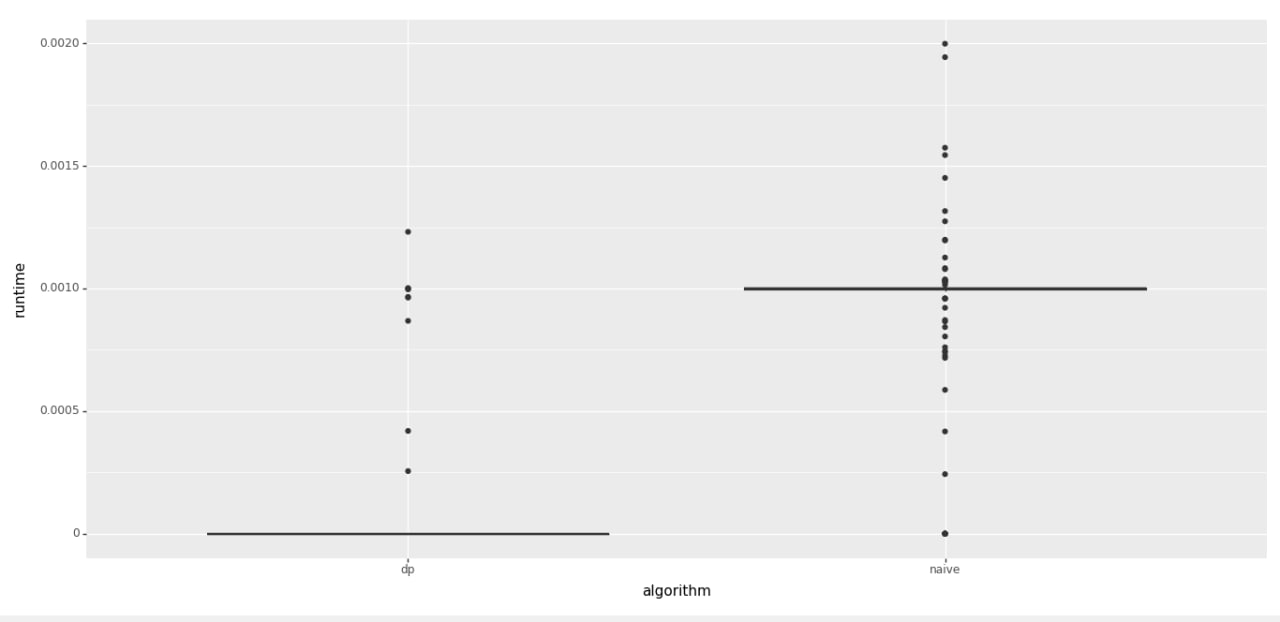
\includegraphics[width=1.0\linewidth]{benchmark_5x5.jpg}
  \caption{Benchmark on a 5x5 image.}
  \end{figure}

\newpage

\begin{figure}[!h]
  \centering
  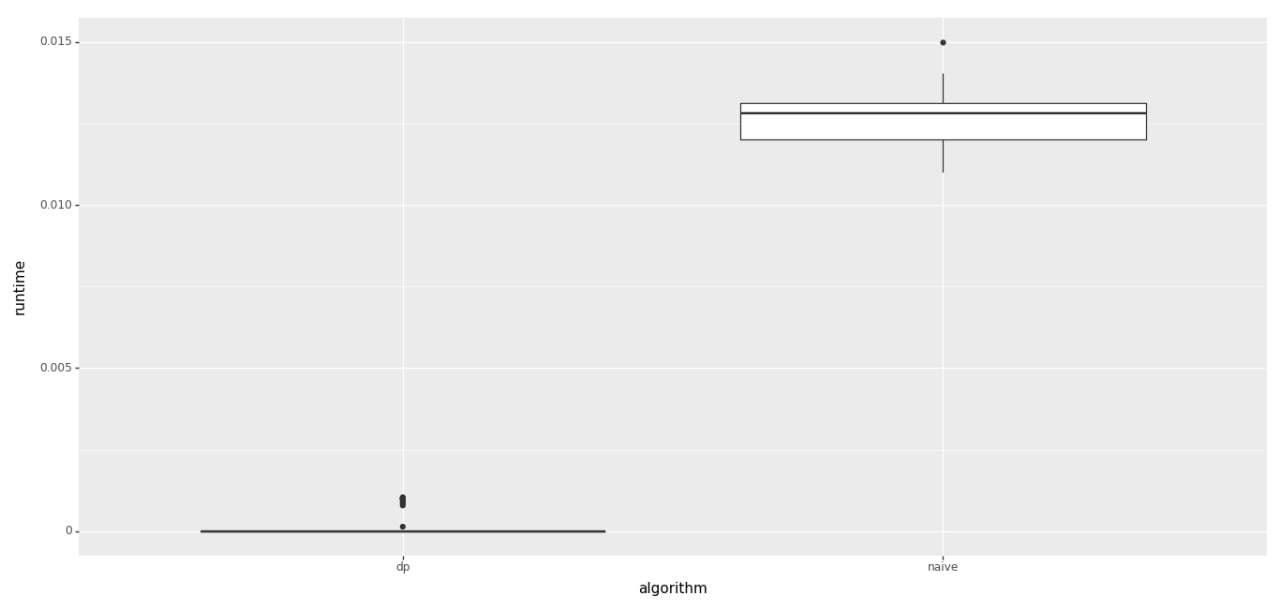
\includegraphics[width=1.0\linewidth]{benchmark_7x7.jpg}
  \caption{Benchmark on a 7x7 image.}
  \end{figure}

\begin{figure}[!h]
  \centering
  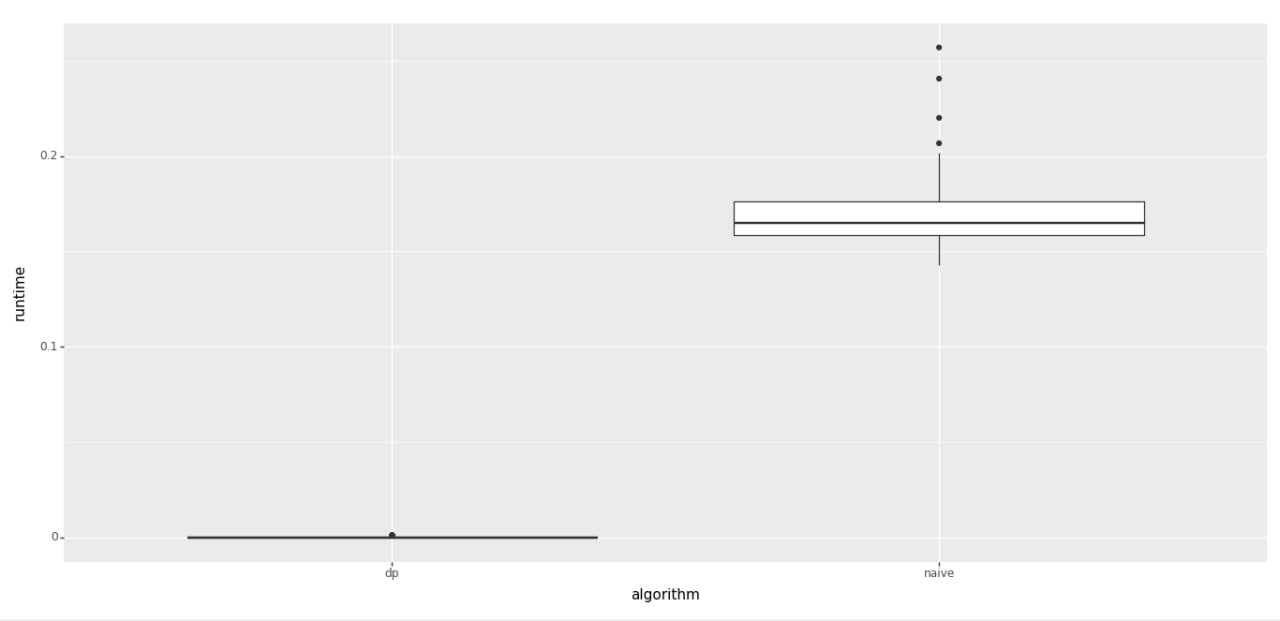
\includegraphics[width=1.0\linewidth]{benchmark_9x9.jpg}
  \caption{Benchmark on a 9x9 image.}
  \end{figure}

\newpage

\begin{figure}[!h]
  \centering
  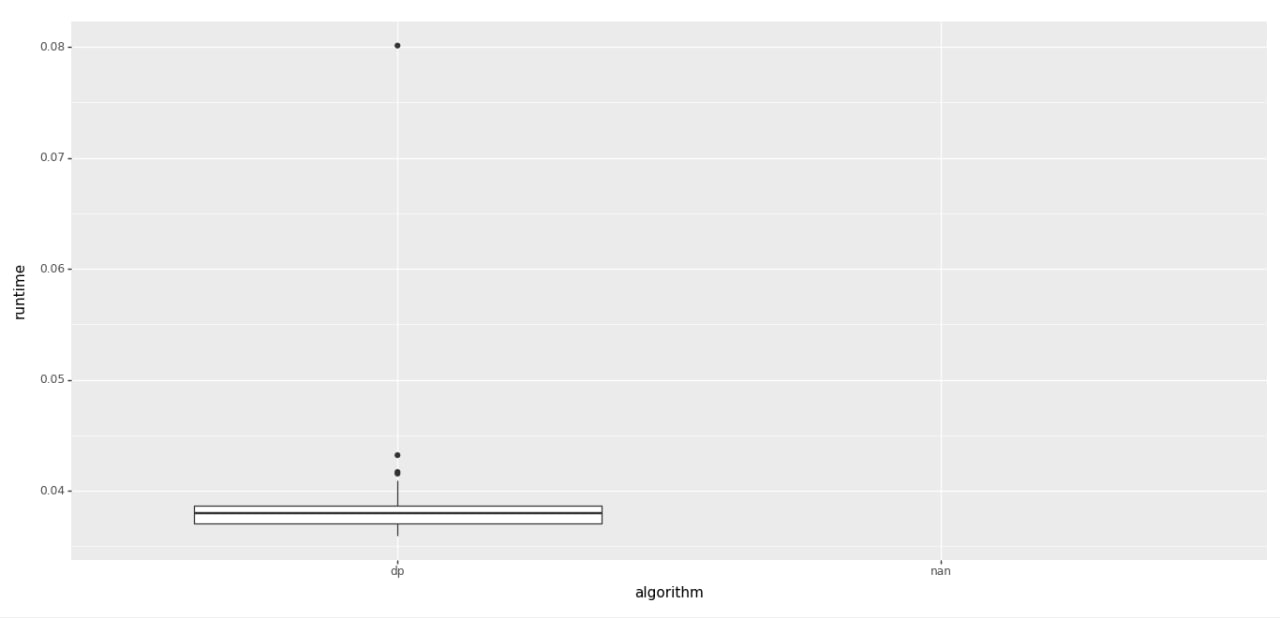
\includegraphics[width=1.0\linewidth]{benchmark_sunset_small.jpg}
  \caption{Benchmark on the small sunset image. (DP only)}
  \end{figure}

\begin{figure}[!h]
  \centering
  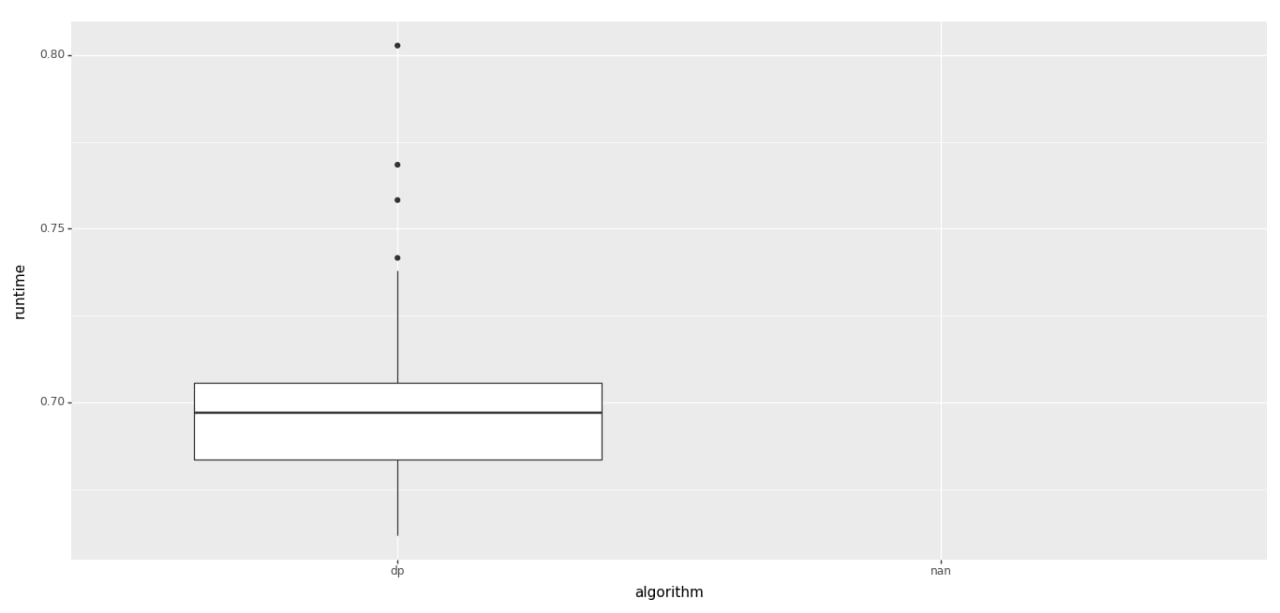
\includegraphics[width=1.0\linewidth]{benchmark_sunset_large.jpg}
  \caption{Benchmark on the large sunset image. (DP only)}
  \end{figure}

For benchmarking, it was done over 100 iterations.
On a smaller image (3 x 3), the time differences between the 
DP and naive solution are almost negligible, with both being concentrated.
As the images get bigger (5 x 5), the timings for the naive solution
start to spread out while the dp solutions are still fairly concentrated.
With larger images (7 x 7) and bigger, naive loses out to dp
in terms of runtime, and we start to see it fall off.
For even larger images, naive takes a long time and may not finish computing in a reasonable amount of time.

\section*{Analysis}

\begin{enumerate}
  \item
    The recurrence for a horizontal seam would be given by the following equation: \\
    \[
       dp[i, j] = min(dp[i - 1, j - 1], dp[i - 1, j], dp[i - 1, j + 1]) + energy(i, j)
    \]
    following the definitions of variables i and j as defined by the problem set.
  \item
    Let n = no. of rows. Let m = no. of columns. 
    Assuming no. of columns $>$ 1, let us assume for simplicity that all
    pixels are the exact same.
    That is to say, the cost to remove any pixel is the same,
    except for those in the edges of an arbitrary high amount (as given in the question).
    Thus, from an arbitrary cell, we have up to 3 potential choices 
    of paths to choose from in order to form our seam.
    As we have n levels in our matrix, and at each level we have 3 choices, 
    the total amount of possible seams in the worst case (where all pixesl are the same)
    could be exponential in terms of $3^n$.
  \item 
    Assume the width and height of the image matrix is given by m x n respectively.
    Thus, the time complexity for the DP solution would be O(mn). \\
    There are a few costly operations in our algorithm: \\
    1. We initially created an array to store the values of the previous row.
    Initializing this array with values would cost O(m). \\
    2. The main bulk of the cost is given in the double for loops,
    where we iterate each cell in the image matrix.
    Since there are n rows, and we iterate m cells in each row,
    the time complexity would be O(mn). \\
    3. The last costly part would be path tracing.
    Here, we reference our dictionary of pointers to previous cells.
    As each cell points to another cell from the previous row,
    we would only need to iterate through n entries.
    Given that the lookup of each entry in a dictionary is constant, 
    the time complexity is thus O(n). \\
    (For our naive method, we omit this step as we are able to
    find the path of the best seam while going down the recursion tree.
    This will save us an iteration to backtrack at the cost of using more space to create more lists) \\
    Hence, the most dominating factor would be O(mn).
  \item 
    Yes. With smaller inputs, the time difference is negligible as 
    there are not many subproblems for the tree to recurse to.
    But with larger inputs, there are many repeated subproblems, 
    and as such we have to spend more time recomputing such subproblems, while it is cached in DP.
    As such, the time taken for naive increases at a faster rate
    as compared to the time taken for DP to increase.
\end{enumerate}

\end{document}
